\documentclass{tufte-handout}

\title{On ultimate: dumps and retaining possession}
\author[James Reynolds]{James Reynolds}

%\date{28 March 2010} % without \date command, current date is supplied

%\geometry{showframe} % display margins for debugging page layout

\usepackage{graphicx} % allow embedded images
  \setkeys{Gin}{width=\linewidth,totalheight=\textheight,keepaspectratio}
  \graphicspath{{graphics/}} % set of paths to search for images
\usepackage{amsmath}  % extended mathematics
\usepackage{booktabs} % book-quality tables
\usepackage{units}    % non-stacked fractions and better unit spacing
\usepackage{multicol} % multiple column layout facilities
\usepackage{lipsum}   % filler text
\usepackage{fancyvrb} % extended verbatim environments
  \fvset{fontsize=\normalsize}% default font size for fancy-verbatim environments

% Standardize command font styles and environments
\newcommand{\doccmd}[1]{\texttt{\textbackslash#1}}% command name -- adds backslash automatically
\newcommand{\docopt}[1]{\ensuremath{\langle}\textrm{\textit{#1}}\ensuremath{\rangle}}% optional command argument
\newcommand{\docarg}[1]{\textrm{\textit{#1}}}% (required) command argument
\newcommand{\docenv}[1]{\textsf{#1}}% environment name
\newcommand{\docpkg}[1]{\texttt{#1}}% package name
\newcommand{\doccls}[1]{\texttt{#1}}% document class name
\newcommand{\docclsopt}[1]{\texttt{#1}}% document class option name
\newenvironment{docspec}{\begin{quote}\noindent}{\end{quote}}% command specification environment

\begin{document}

\maketitle% this prints the handout title, author, and date



%\printclassoptions

Defence wins games 
and offence loses them 
because,   
having more turnovers 
than the other team 
results in
scoring fewer goals\footnote{
There are 
some edge cases 
(e.g. so windy that 
no one can score 
upwind, so the
flip decides the game.)}. 
Hence, 
being able 
to retain possession 
is important\footnote{
More important than getting 
a big layout block on 
defence? Possibly, 
because at that point 
the job 
is only half done - 
your team still 
needs to convert 
the block into a goal!}. 
Being able 
to throw a dump 
is therefore a 
key skill for any
ultimate player. 
If you're a handler 
being able to 
set up for 
and then receive a dump 
is vital too\footnote{
With the rare exception of 
if you are on the defence team 
and the team's strategy is to 
score as soon as possible 
after getting a turnover 
(e.g. D and huck and D).}


This document is  
a two-pager about 
throwing or 
receiving a dump pass\footnote{
This
is part of a series, 
available at
\url{https://github.com/James-Reynolds/Ultimate-strategy-and-tactics}.}. 
It first discusses 
what a dump is 
and why it is important. 
Positioning for the dump 
is discussed, 
followed by how to 
engage with 'the dump'
and complete a dump pass. 
Finally, using 
dumps to generate 
offensive opportunities 
is discussed. 

\section{What is a dump and why is it important?}\label{sec:what_is_a_dump}
What is a dump\footnote{
A backwards pass? 
Sometimes.  
A short pass? 
Often. 
A pass back to a handler? 
Usually.}? 
It can mean a lot of things, 
but usually 
it refers to 
'dumping it' 
back to one of the handlers 
so as to 
reset the stall count 
and retain possession 
of the disc.  
In short,
it is 
a high-percentage 
pass, 
made to reset 
the stall count 
and so retain possession\footnote{
There are three ways 
for a turnover to occur:
1) the stall count reaches 10; 
2) a pass is incomplete; or
3) a pass is intercepted. 
Throwing a dump deals 
with all three as:
it gets the stall count back to zero; 
dumps are 
generally easier throws 
to make; and 
there is not much that a defender 
can do about a well thrown dump, 
as they are difficult to intercept. }.  
It is important because 
it impacts, 
and to an extend dictates, 
whether your team can 
play low-risk, high-completion 
offense. 
With an effective dump-set 
your team can retain possession
and wait for  
good opportunities.  
Without a reliable dump-set, 
you'll likely 
have to play higher-risk 
offence\footnote{
Huck-and-zone anyone? 
Not that there is anything 
wrong with huck-and-zone 
if it is working. 
Just that it 
will not 
work against teams
who don't turn the disc over much.}.  
Unfortunately, it's time for...

\subsection{...some probability}
\label{sec:probability}
The probability 
of scoring  
is a function of 
the number of passes made 
and the completion rate of 
each of those passes\footnote{
For example, 
you might catch the pull 
and then immediately 
throw it deep 
to the endzone.
Maybe there is a 
40\% chance 
of someone on your team 
catching it for a goal. 
Alternatively, 
your team might 
score with five 
lower-risk throws. 
However, if each has 
a 85\% completion rate
the chance of scoring is only 44\%, 
as 
\begin{equation} 0.85^5 = 0.44 \end{equation}
That single high-risk 
throw isn't looking to bad actually...}. 
Different players 
on your team 
will have 
different completion rates, 
and these too 
will be impacted by 
whether they are 
taking high- or low-risk 
options, 
so it all gets a bit complicated.
But, 
in general, 
if the completion rate 
of your entire team goes up, 
your more experienced throws 
will likely be able to take 
less risky options\footnote{
Again, returning to the one high-risk  
versus five lower-risk throws example, 
if the completion rate goes up 
to 90\%, we are now looking at: 
\begin{equation} 0.9^5 = 0.59 \end{equation}
...and suddenly that 40\% huck 
isn't looking too good anymore.
}.  


\begin{margintable}
\caption{Completion rates 1}
\begin{tabular}{|l|r r r|}
\hline
 & \multicolumn{3}{|c|}{Completion rate} \\
 \hline
Players & Huck & Regular & Dump \\
O1, O2, O3, O4 & - & 50\% & 60\% \\
O5, O6, O7 & 40\% & 80\% & 90\%\\
\hline
\end{tabular}
\end{margintable}

If a handler has the disc 
one option 
might be 
to attempt 
a huck  for a goal 
(40\% chance of 
success).  
Alternatively, a 
(non-huck) 
regular throw 
to a cutter 
might advance the disc, 
(80\% completion). 
However, if this
does not score, 
the cutter 
will then have to 
throw another forward pass 
(40\% completion rate = 32\% overall),
or a dump (60\% completion rate = 48\% overall). 
Every pass increases 
the overall risk of a turn, 
and the original 
40\% chance
of a huck succeeding 
is already starting to look pretty good\footnote{
Essentially, if the 
dump completion 
rate is low the handler 
might as well 
have a shot for 
a goal 
given that if they take 
a lower risk option 
it's about the same overall chance 
of turning over anyway.} 

\begin{margintable}
\caption{Completion rates 2}
\begin{tabular}{|l|r r r|}
\hline
 & \multicolumn{3}{|c|}{Completion rate} \\
 \hline
Players & Huck & Regular & Dump \\
O1, O2, O3, O4 & - & 50\% & 80\% \\
O5, O6, O7 & 60\% & 80\% & 90\%\\
\hline
\end{tabular}
\end{margintable}

Now, compare to the 
situation shown in Table 2, 
with the cutters (O1-4) 
having a 80\% completion rate 
for a dump.
That 40\% huck isn't looking 
very good any more, 
given that a handler-cutter (80\%) 
and cutter-dump (80\%) is overall 
64\%
Table 2, therefore, 
suggests that, 
with the higher dump completion rate
amongst the cutters, 
the handlers can
be a bit more conservative 
when hucking\footnote{
The handler huck 
percentage is show 
as having increased 
to 60\%, 
suggesting that the handlers
will be looking off the 
riskier hucks. 
The point, 
in effect, 
being that 
if you (as a cutter) 
can improve 
your dumping 
it has flow-on benefits 
for throws by others 
and the team as a whole.}.






\section{Positioning}
\label{sec:positioning}

\section{Engaging and completing}
\label{sec:engaging}

\section{Gaining an advantage from dumping}
\label{sec:engaging}



\begin{marginfigure}%
  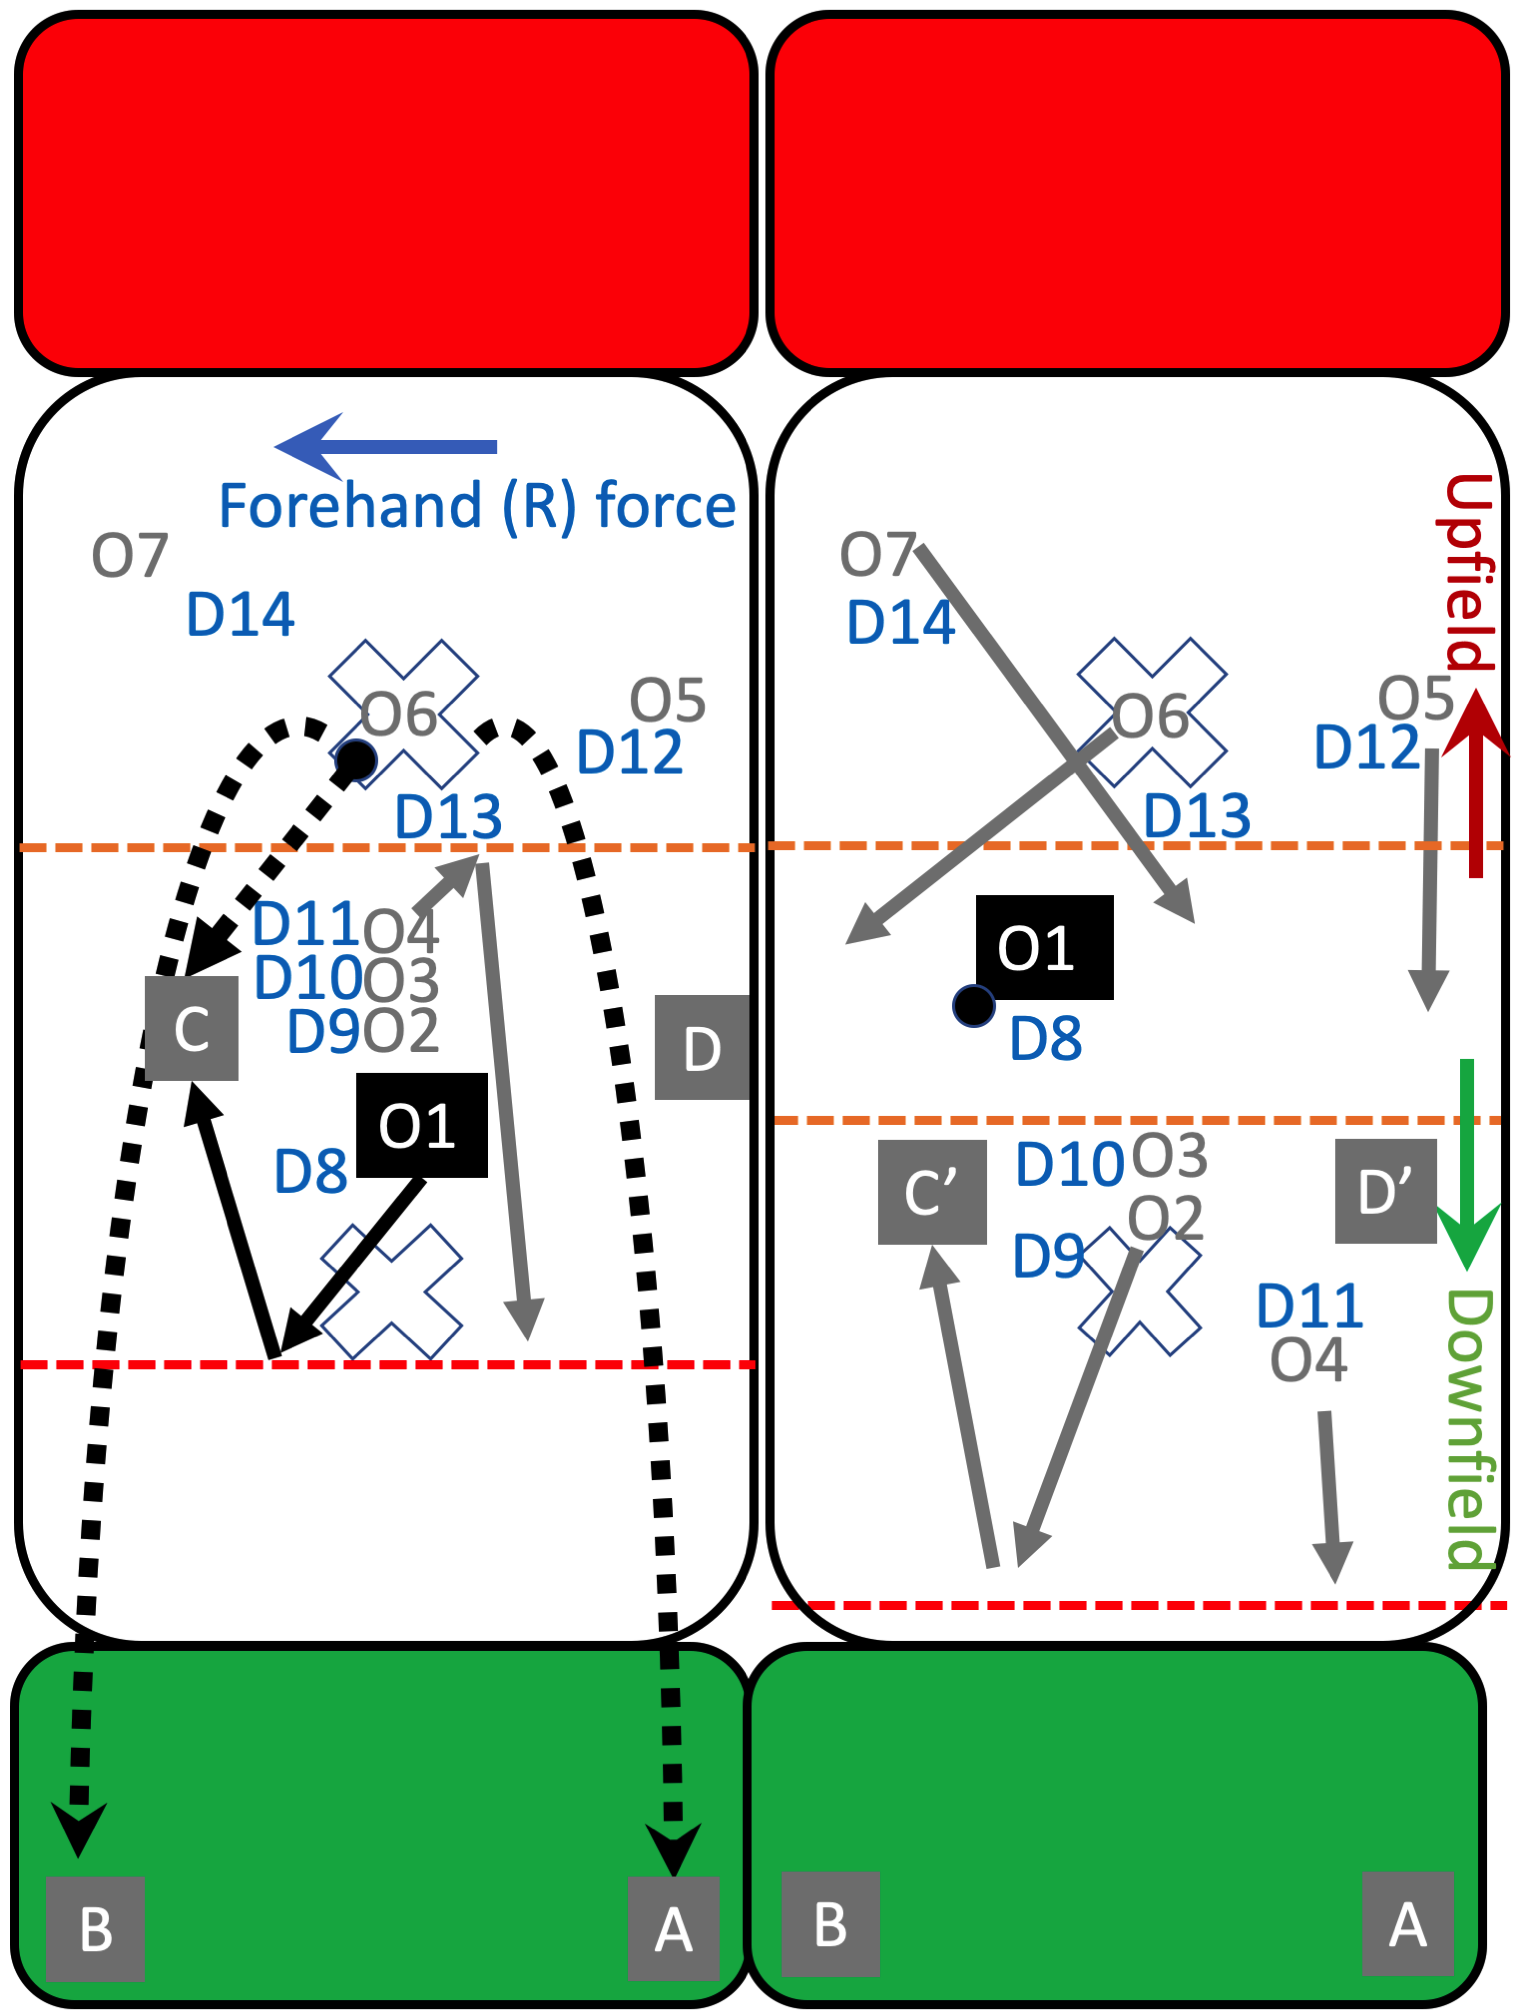
\includegraphics[width=\linewidth]{O1-vertical}
  \caption{Vertical stack: 
  starting position (left),
  and development (right)}
  \label{fig:O1-vertical}
\end{marginfigure}


\end{document}
